\subsection{Mock Interview Sessions}
\label{sec:impl_interviews}

The mock interview subsystem assesses a learner through a structured question-and-answer session. Teachers configure and publish the interview in advance, including its questions, learning outcomes, and assessment rules. Published settings remain stable for the duration of a learner session.

\paragraph{Main handling flow}
The learner completes onboarding, then answers each interview question through typed text or optional audio input. The system records the turn, analyses the response, and selects a follow-up or next question. This loop continues until the configured interview scope is complete, after which terminal evaluation produces the final result and feedback.

\begin{figure}[H]
    \centering
    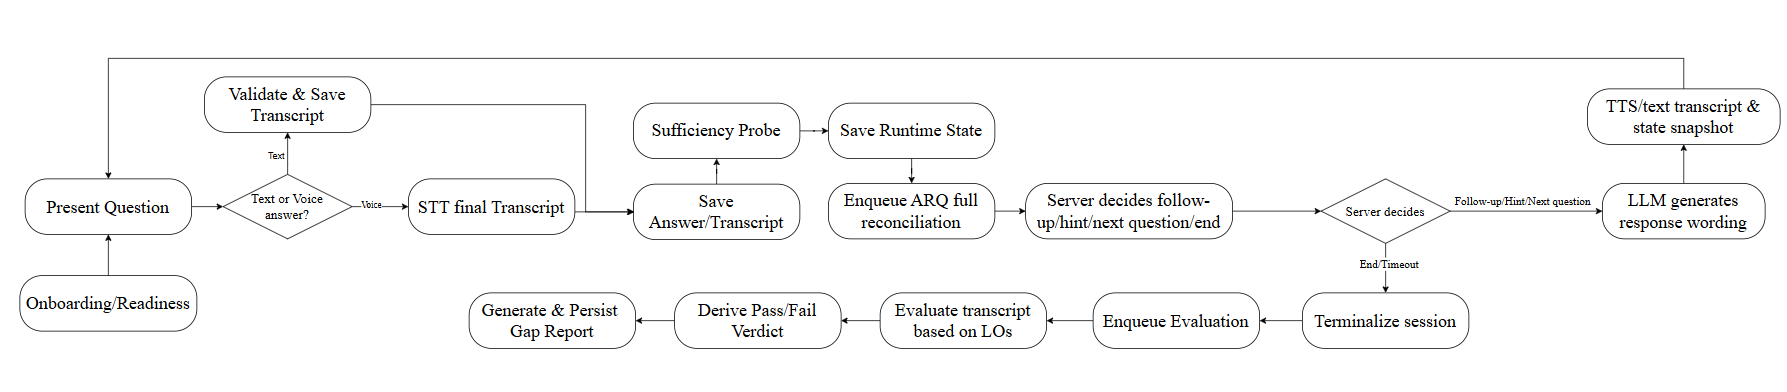
\includegraphics[width=0.95\textwidth]{graphics/act-diagrams/act_mock_interview_flow.png}
    \caption{Activity Diagram: Mock Interview Main Handling Flow.}
    \label{fig:impl-mock-interview-flow}
\end{figure}

In-session processing supports the conversation, while terminal evaluation determines the assessment result. Learners receive their result and improvement guidance. Authorised teachers can review the supporting session record and assessment information.
